针对多变量观测条件下的 CO$_2$ 浓度单步预测，我们采用 GRU 多种子集成与岭回归加权融合的方法。图~\ref{fig:method-overview} 展示的是该方法的整体框架。标准化后的观测窗口分别输入两条分支：GRU 分支通过门控状态递推刻画非线性依赖，并对各成员预测取均值；岭回归分支将窗口按行展平后进行线性预测。两条分支的输出在标准化空间内加权融合，经反标准化得到以 ppm 为单位的 CO$_2$ 浓度。

\begin{figure*}[t]
  \centering
  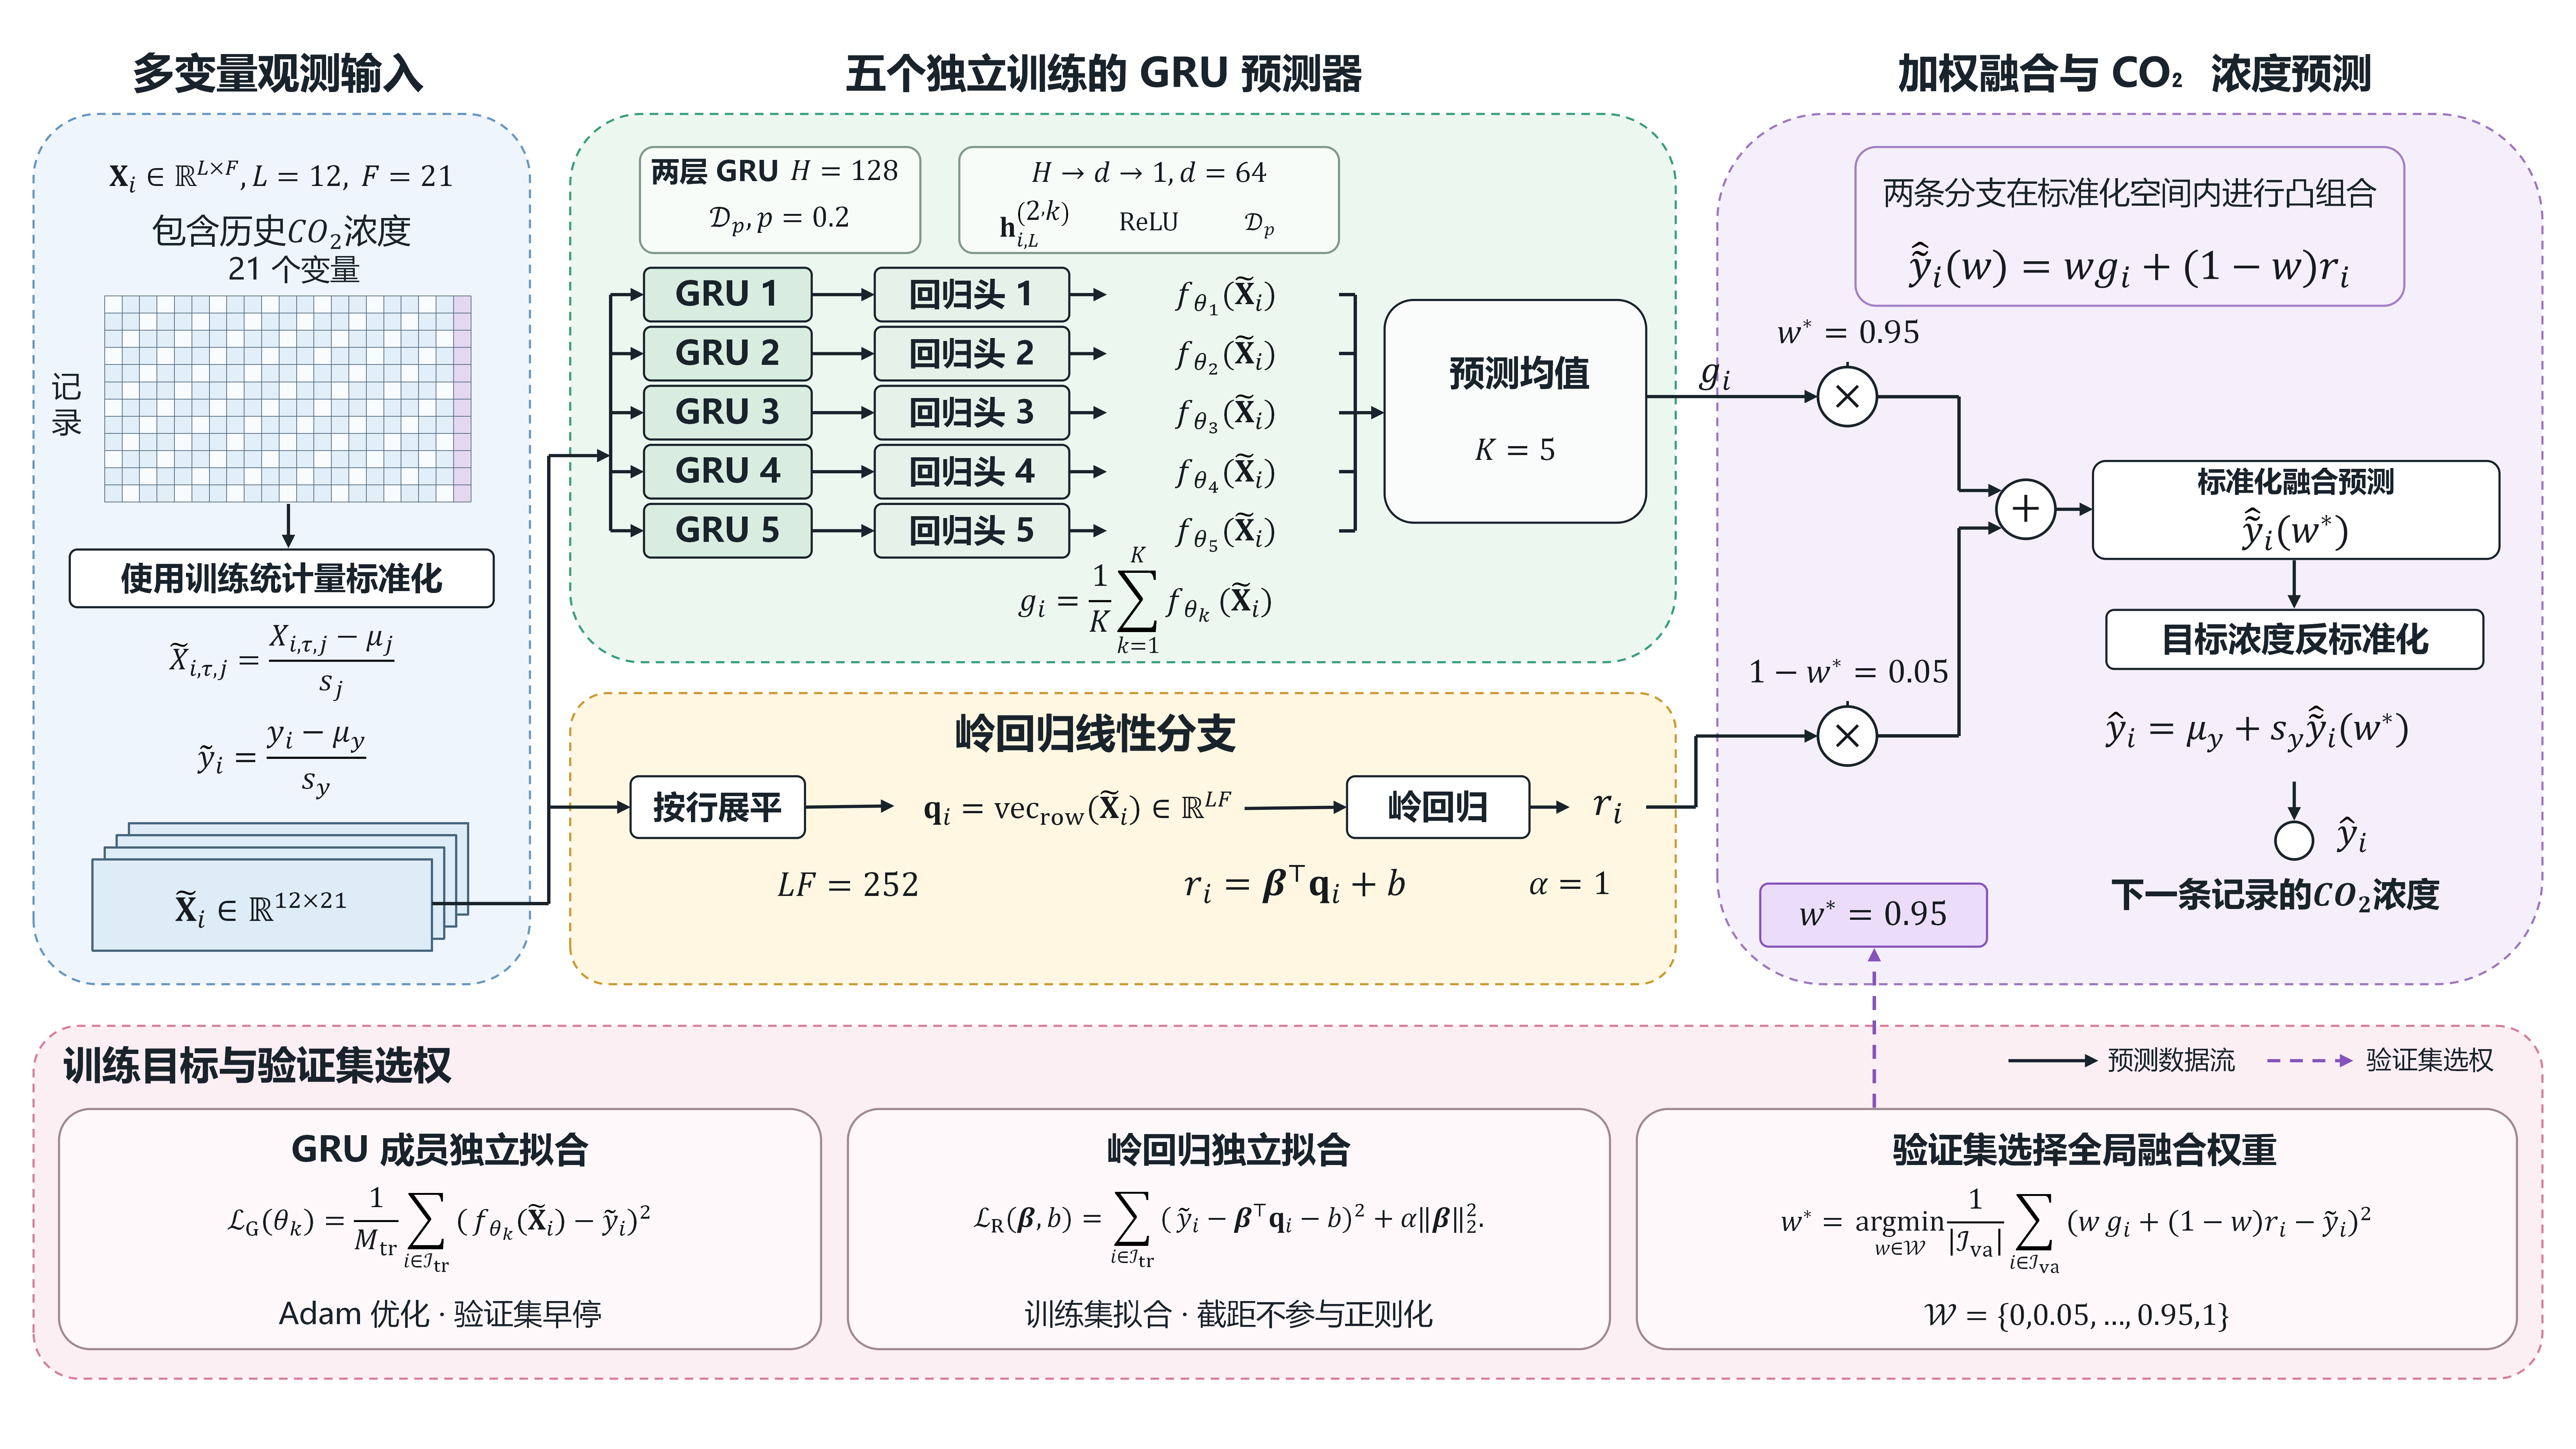
\includegraphics[width=\textwidth,trim=62bp 135bp 62bp 102bp,clip]{figures/model_overview.png}
  \Description{GRU 多种子集成与岭回归融合方法的整体框架，包括多变量观测标准化、GRU 成员预测取均值、岭回归预测、加权融合与目标浓度反标准化，以及两条分支的损失函数和验证集选权流程。}
  \caption{GRU 多种子集成与岭回归融合的 CO$_2$ 浓度预测框架}
  \label{fig:method-overview}
\end{figure*}

\subsection{任务定义}
\label{sec:method:problem}

设第 $t$ 条多变量观测为 $\mathbf{x}_t\in\mathbb{R}^{F}$，其中 $F$ 为特征维度。预测目标为 CO$_2$ 浓度 $y_t=x_{t,j_*}$，$j_*$ 表示目标特征的索引。令输入窗口长度为 $L$，模型根据此前 $L$ 条观测预测目标浓度：
\begin{equation}
    \mathbf{X}_t=
    [\mathbf{x}_{t-L},\ldots,\mathbf{x}_{t-1}]^\top
    \in\mathbb{R}^{L\times F},
    \qquad \widehat{y}_t=f(\mathbf{X}_t).
    \label{eq:window}
\end{equation}

\subsection{共享特征与目标标准化}
\label{sec:method:normalization}


气象变量的量纲与数值尺度存在差异，因此两条分支统一使用标准化后的窗口。记第 $j$ 个特征的均值与标准差为 $\mu_j$ 和 $s_j$，输入与目标的变换为
\begin{equation}
    \widetilde{X}_{i,\tau,j}=\frac{X_{i,\tau,j}-\mu_j}{s_j},
    \qquad
    \widetilde{y}_i=\frac{y_i-\mu_y}{s_y},
    \label{eq:standardization}
\end{equation}
其中 $\mu_y=\mu_{j_*}$、$s_y=s_{j_*}$，即标签与输入中的 CO$_2$ 特征使用相同的缩放尺度。两条分支的目标尺度保持一致，为后续融合预测值提供统一的数值基础。统计量的估计方式见第~\ref{sec:exp:preprocessing} 节。

\subsection{门控循环预测器}
\label{sec:method:gru}

非线性分支采用门控循环单元（GRU）\citep{cho2014learning}，根据当前观测调节历史隐藏状态对预测表示的影响。每个预测器包含两层单向 GRU，隐藏维度均为 $H$。对其中一层，记窗口位置 $\tau$ 的输入为 $\mathbf{u}_\tau$，前一位置的隐藏状态为 $\mathbf{h}_{\tau-1}\in\mathbb{R}^{H}$。重置门与更新门分别为
\begin{align}
    \mathbf{r}_\tau&=\sigma\bigl(
    \mathbf{W}_{ir}\mathbf{u}_\tau+\mathbf{b}_{ir}
    +\mathbf{W}_{hr}\mathbf{h}_{\tau-1}+\mathbf{b}_{hr}\bigr),
    \label{eq:reset}\\
    \mathbf{z}_\tau&=\sigma\bigl(
    \mathbf{W}_{iz}\mathbf{u}_\tau+\mathbf{b}_{iz}
    +\mathbf{W}_{hz}\mathbf{h}_{\tau-1}+\mathbf{b}_{hz}\bigr).
    \label{eq:update}
\end{align}
候选状态和隐藏状态更新为\citep{pytorchgru}：
\begin{align}
    \mathbf{n}_\tau
    &=\tanh\!\left(
      \begin{aligned}
        &\mathbf{W}_{in}\mathbf{u}_\tau+\mathbf{b}_{in}\\[-2pt]
        &{}+\mathbf{r}_\tau\odot
          \bigl(\mathbf{W}_{hn}\mathbf{h}_{\tau-1}
          +\mathbf{b}_{hn}\bigr)
      \end{aligned}
      \right),
    \label{eq:candidate}\\[3pt]
    \mathbf{h}_\tau
    &=(\mathbf{1}-\mathbf{z}_\tau)\odot\mathbf{n}_\tau
      +\mathbf{z}_\tau\odot\mathbf{h}_{\tau-1}.
    \label{eq:state}
\end{align}
其中，$\sigma$ 为 Sigmoid 函数，$\odot$ 表示逐元素乘法。重置门控制历史状态在候选状态中的参与程度，更新门控制旧状态的保留比例。式~\eqref{eq:candidate} 先对历史状态进行仿射变换，再施加重置门。

第一层接收标准化特征向量，第二层接收经过 Dropout\citep{srivastava2014dropout} 的第一层输出：
\begin{equation}
    \mathbf{u}_{i,\tau}^{(1)}=\widetilde{\mathbf{x}}_{i,\tau},
    \qquad
    \mathbf{u}_{i,\tau}^{(2)}=
    \mathcal{D}_{p}(\mathbf{h}_{i,\tau}^{(1)}),
    \label{eq:stacking}
\end{equation}
这里 $\widetilde{\mathbf{x}}_{i,\tau}$ 为第 $i$ 个标准化窗口在位置 $\tau$ 的特征向量，$\mathcal{D}_p$ 表示丢弃概率为 $p$ 的 Dropout 算子，作用于两层之间的输出。

第二层最后一个位置的隐藏状态用于生成浓度预测。对第 $k$ 个集成成员，回归头依次执行全连接变换、ReLU、Dropout 和线性输出：
\begin{align}
    \mathbf{a}_i^{(k)}&=\operatorname{ReLU}
    (\mathbf{W}_{1}^{(k)}\mathbf{h}_{i,L}^{(2,k)}
    +\mathbf{b}_{1}^{(k)}),
    \label{eq:head_hidden}\\
    f_{\theta_k}(\widetilde{\mathbf{X}}_i)&=
    \mathbf{W}_{2}^{(k)}\mathcal{D}_{p}(\mathbf{a}_i^{(k)})+b_{2}^{(k)},
    \label{eq:head_output}
\end{align}
其中 $\mathbf{W}_{1}^{(k)}\in\mathbb{R}^{d\times H}$，$\mathbf{W}_{2}^{(k)}\in\mathbb{R}^{1\times d}$，$d$ 为回归头的隐藏维度，$\theta_k$ 表示第 $k$ 个预测器的参数。输出为标准化后的标量浓度，不施加概率范围约束。

\subsection{循环预测器的损失与集成}
\label{sec:method:ensemble}

记训练样本索引集为 $\mathcal{I}_{\mathrm{tr}}$，样本数为 $M_{\mathrm{tr}}=|\mathcal{I}_{\mathrm{tr}}|$。各 GRU 成员分别使用标准化标签上的均方误差（MSE）作为目标：
\begin{equation}
    \mathcal{L}_{\mathrm{G}}(\theta_k)=
    \frac{1}{M_{\mathrm{tr}}}
    \sum_{i\in\mathcal{I}_{\mathrm{tr}}}
    \bigl(f_{\theta_k}(\widetilde{\mathbf{X}}_i)-\widetilde{y}_i\bigr)^2.
    \label{eq:gru_loss}
\end{equation}
集成包含 $K$ 个预测器，对各成员的标准化预测取算术平均：
\begin{equation}
    g_i=\frac{1}{K}\sum_{k=1}^{K}
    f_{\theta_k}(\widetilde{\mathbf{X}}_i).
    \label{eq:ensemble}
\end{equation}
该操作在预测空间整合多个非线性映射。

\subsection{正则化线性预测分支}
\label{sec:method:ridge}

线性分支为窗口内不同时间位置的观测变量分别设置回归系数，通过加权求和预测目标浓度。将标准化窗口按行展平为 $LF$ 维向量后，采用岭回归\citep{hoerl1970ridge} 计算预测：
\begin{equation}
    \mathbf{q}_i=\operatorname{vec}_{\mathrm{row}}
    (\widetilde{\mathbf{X}}_i)\in\mathbb{R}^{LF},
    \qquad r_i=\boldsymbol{\beta}^{\top}\mathbf{q}_i+b.
    \label{eq:ridge_prediction}
\end{equation}
岭回归与 GRU 使用相同的输入观测和标准化标签，其系数与截距通过下式拟合：
\begin{equation}
    \begin{split}
    \mathcal{L}_{\mathrm{R}}(\boldsymbol{\beta},b)
    =&\sum_{i\in\mathcal{I}_{\mathrm{tr}}}
    (\widetilde{y}_i-\boldsymbol{\beta}^{\top}\mathbf{q}_i-b)^2\\
    &+\alpha\lVert\boldsymbol{\beta}\rVert_2^2.
    \end{split}
    \label{eq:ridge_loss}
\end{equation}
正则项约束系数幅度，以处理滞后输入之间的相关性，截距 $b$ 不参与惩罚。

\subsection{加权融合与浓度还原}
\label{sec:method:fusion}

两条分支的预测通过凸组合得到标准化融合预测：
\begin{equation}
    \widehat{\widetilde{y}}_i(w)=w g_i+(1-w)r_i,
    \qquad w\in[0,1],
    \label{eq:fusion}
\end{equation}
其中 $w$ 控制 GRU 集成的贡献，$1-w$ 为岭回归的权重。所有样本共享同一个组合系数，两个端点分别对应单独使用岭回归或 GRU 集成。记最终采用的组合系数为 $w^*$，其选择过程见第~\ref{sec:exp:training} 节。利用目标统计量将融合结果还原为浓度：
\begin{equation}
    \widehat{y}_i=\mu_y+s_y
    \left[w^*\frac{1}{K}\sum_{k=1}^{K}
    f_{\theta_k}(\widetilde{\mathbf{X}}_i)
    +(1-w^*)r_i\right].
    \label{eq:final_prediction}
\end{equation}
